\documentclass[12pt]{beamer}
\usepackage[utf8]{inputenc}
\usepackage[T1]{fontenc}
\usepackage{lmodern}
\usepackage{amsmath}
\usepackage{graphicx}
\usepackage{tikz}
\usetikzlibrary{arrows.meta, intersections}

\usetheme{Madrid}
\usecolortheme{seahorse}

\title[Iterações Lineares e Pontos Fixos]{\textbf{Iterações Lineares e Pontos Fixos}}
\subtitle{Live Não Trivial - Teoria do Caos}
\author[Hassan S. Primo]{Hassan S. Primo\\\small Projeto Não Trivial}
\date{}

\begin{document}

\begin{frame}
  \titlepage
  \begin{tikzpicture}[remember picture,overlay]
    \node[anchor=north east, inner sep=20pt] at (current page.north east) 
    {\includegraphics[width=2cm]{logo.png}}; % Adicione seu logo
  \end{tikzpicture}
\end{frame}

\section{Abertura}

\begin{frame}{Boas-vindas!}
  \begin{columns}
    \column{0.6\textwidth}
    \begin{block}{}
      \begin{center}
        \Large\textbf{Bem-vindos à Live!}
      \end{center}
    \end{block}
    
    \begin{itemize}
      \item Repetição como ferramenta matemática
      \item Ordem oculta no aparente caos
      \item Filosofia da estabilidade
    \end{itemize}
    
    \vspace{5mm}
    \textit{"A mesma causa pode produzir diferentes efeitos dependendo de como interage consigo mesma"}
    
    \column{0.4\textwidth}
    \includegraphics[width=\textwidth]{iteracao.png} % Imagem ilustrativa
  \end{columns}
\end{frame}

\section{Conceitos Fundamentais}

\begin{frame}{Iteração Linear: A Essência}
  \[
  x_{n+1} = a \cdot x_n + b
  \]
  
  \begin{columns}
    \column{0.5\textwidth}
    \begin{exampleblock}{Caso Atraente}
      \[
      a = 0.5,\; x_0 = 10
      \]
      \begin{tikzpicture}[scale=0.6]
        \draw[->] (0,0) -- (4,0) node[right] {$n$};
        \draw[->] (0,0) -- (0,3) node[above] {$x_n$};
        \draw[red, thick] plot coordinates {(0,2.5) (1,1.25) (2,0.625) (3,0.3125)};
      \end{tikzpicture}
    \end{exampleblock}

    \column{0.5\textwidth}
    \begin{alertblock}{Caso Repulsivo}
      \[
      a = 1.5,\; x_0 = 1
      \]
      \begin{tikzpicture}[scale=0.6]
        \draw[->] (0,0) -- (4,0) node[right] {$n$};
        \draw[->] (0,0) -- (0,3) node[above] {$x_n$};
        \draw[blue, thick] plot coordinates {(0,0.5) (1,1.5) (2,2.5) (3,3.5)};
      \end{tikzpicture}
    \end{alertblock}
  \end{columns}
\end{frame}

\begin{frame}{Ponto Fixo: O Equilíbrio Escondido}
  \begin{columns}
    \column{0.5\textwidth}
    \[
    f(x^*) = x^* \Rightarrow x^* = \frac{b}{1 - a}
    \]
    
    \begin{itemize}
      \item Atração vs. Repulsão
      \item Sensibilidade aos parâmetros
      \item Analogia com equilíbrios na vida real
    \end{itemize}
    
    \column{0.5\textwidth}
    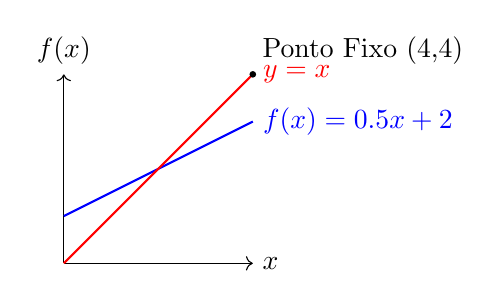
\begin{tikzpicture}[scale=0.6]
      \draw[->] (0,0) -- (4,0) node[right] {$x$};
      \draw[->] (0,0) -- (0,4) node[above] {$f(x)$};
      \draw[thick,blue] (0,1) -- (4,3) node[right] {$f(x) = 0.5x + 2$};
      \draw[thick,red] (0,0) -- (4,4) node[right] {$y = x$};
      \fill (4,4) circle (2pt) node[above right] {Ponto Fixo (4,4)};
    \end{tikzpicture}
  \end{columns}
\end{frame}

\section{Estabilidade e Caos}

\begin{frame}{A Dança da Estabilidade}
  \centering
  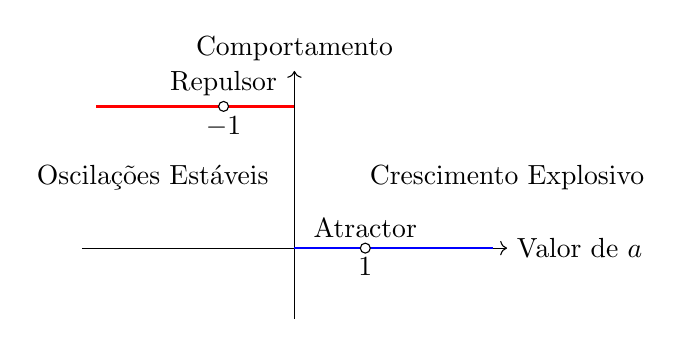
\begin{tikzpicture}[scale=0.9]
    \draw[->] (-3,0) -- (3,0) node[right] {Valor de $a$};
    \draw[->] (0,-1) -- (0,2.5) node[above] {Comportamento};
    
    \draw[thick,red] (-2.8,2) -- (-1,2) node[black,above] {Repulsor} -- (0,2);
    \draw[thick,blue] (0,0) -- (1,0) node[black,above] {Atractor} -- (2.8,0);
    
    \draw[fill=white] (-1,2) circle (2pt) node[below] {$-1$};
    \draw[fill=white] (1,0) circle (2pt) node[below] {$1$};
    
    \node at (-2,1) {Oscilações Estáveis};
    \node at (3,1) {Crescimento Explosivo};
  \end{tikzpicture}
  
  \vspace{5mm}
  \[
  |a| < 1 \Rightarrow \text{Estabilidade} \quad vs \quad |a| > 1 \Rightarrow \text{Caos}
  \]
\end{frame}

\section{Engajamento e Encerramento}

\begin{frame}{Reflexão Coletiva}
  \begin{columns}
    \column{0.6\textwidth}
    \begin{block}{Perguntas para o Chat}
      \begin{itemize}
        \item Qual hábito seu é um ponto fixo estável?
        \item Se sua vida fosse uma iteração, que valor de $a$ teria?
        \item O que acontece quando $a = 1$?
      \end{itemize}
    \end{block}
    
    \begin{exampleblock}{Atividade Prática}
      Calcule o ponto fixo para:
      \[
      x_{n+1} = 0.8x_n + 5
      \]
      \textit{Primeiros 3 que acertarem ganham destaque!}
    \end{exampleblock}

    \column{0.4\textwidth}
    \includegraphics[width=\textwidth]{caos.png} % Imagem de fractal ou sistema caótico
  \end{columns}
\end{frame}

\begin{frame}{Encerramento}
  \centering
  \begin{beamercolorbox}[sep=8pt,center]{title}
    \usebeamerfont{title}\textbf{Continue Explorando!}
  \end{beamercolorbox}
  
  \vspace{5mm}
  \begin{itemize}
    \item Newsletter do Não Trivial
    \item Desafios semanais no Instagram
    \item Próxima live: Sistemas Não-Lineares
  \end{itemize}
  
  \vspace{8mm}
  \begin{block}{}
    \centering
    \Large\textit{"A ordem nasce do caos quando compreendemos suas regras"}
  \end{block}
\end{frame}

\end{document}
